 \documentclass[12pt,a4paper]{article}

\usepackage{graphicx}% Include figure files
\usepackage{dcolumn}% Align table columns on decimal point
\usepackage{bm}% bold math
%\usepackage{hyperref}% add hypertext capabilities
%\usepackage[mathlines]{lineno}% Enable numbering of text and display math
%\linenumbers\relax % Commence numbering lines

%\usepackage[showframe,%Uncomment any one of the following lines to test 
%%scale=0.7, marginratio={1:1, 2:3}, ignoreall,% default settings
%%text={7in,10in},centering,
%%margin=1.5in,
%%total={6.5in,8.75in}, top=1.2in, left=0.9in, includefoot,
%%height=10in,a5paper,hmargin={3cm,0.8in},
%]{geometry}

\usepackage{multicol}%Para hacer varias columnas
\usepackage{multicol,caption}
\usepackage{multirow}
\usepackage{cancel}
\usepackage{hyperref}
\hypersetup{
    colorlinks=true,
    linkcolor=blue,
    filecolor=magenta,      
    urlcolor=cyan,
}

\setlength{\topmargin}{-1.0in}
\setlength{\oddsidemargin}{-0.3pc}
\setlength{\evensidemargin}{-0.3pc}
\setlength{\textwidth}{6.75in}
\setlength{\textheight}{9.5in}
\setlength{\parskip}{0.5pc}

\usepackage[utf8]{inputenc}
\usepackage{expl3,xparse,xcoffins,titling,kantlipsum}
\usepackage{graphicx}
\usepackage{xcolor} 
\usepackage{siunitx}
\usepackage{nopageno}
\usepackage{lettrine}
\usepackage{caption}
\renewcommand{\figurename}{Figura}
\usepackage{float}
\renewcommand\refname{Bibliograf\'ia}
\usepackage{amssymb}
\usepackage{amsmath}
\usepackage[rightcaption]{sidecap}
\usepackage[spanish]{babel}

\providecommand{\abs}[1]{\lvert#1\rvert}
\providecommand{\norm}[1]{\lVert#1\rVert}
\newcommand{\dbar}{\mathchar'26\mkern-12mu d}

% CABECERA Y PIE DE PÁGINA %%%%%
\usepackage{fancyhdr}
\pagestyle{fancy}
\fancyhf{}

\begin{document}

Macías Márquez Misael Iván

\begin{enumerate}



%%%1%%%



\item Encuentre las trayectorias y las leyes de movimiento de una partícula que se mueve bajo el campo de fuerzas centrales,

\begin{equation*}
    U(r) = \left\{\begin{matrix}
    - V & r<R \\
    0 & r> R
    
    \end{matrix}\right.
\end{equation*}

con $V > 0$, para diferentes valores del momento angular y la energía.

\textbf{Sol:}

Dado que tenemos un problema de fuerza central, el lagrangiano del sistema queda descrito por

\begin{equation*}
    L = \frac{1}{2} m \dot{r}^2 + \frac{1}{2}m r^2 \dot{\phi}^2 - U(r)
\end{equation*}

y como $L$ no depende de $\phi$ y $t$ explícitamente, entonces

\begin{equation*}
    \frac{\partial L}{\partial \dot{\phi}} = cte = M = m r^2 \dot{\phi}
\end{equation*}

o bien

\begin{equation*}
    \dot{\phi}^2 = \left(\frac{M}{mr^2}\right)^2 = \frac{M^2}{m^2 r^4}
\end{equation*}

ahora como la energía total ($E$) se conserva

\begin{equation*}
    E = T + U = \frac{1}{2} m \dot{r}^2 + \frac{1}{2} m r^2 \dot{\phi}^2 + U(r) = \frac{1}{2} m \dot{r}^2 + \frac{1}{2} m r^2 \frac{M^2}{m^2 r^4} + U(r)
\end{equation*}

y despejando $\dot{r}$

\begin{equation*}
    \dot{r} = \sqrt{\frac{2}{m}(E-U(r)) - \frac{M^2}{m^2 r^2}}
\end{equation*}

o también

\begin{equation*}
    t = \int \frac{dr}{\sqrt{\frac{2}{m}(E-U(r)) - \frac{M^2}{m^2 r^2}}}
\end{equation*}

\begin{equation*}
    \phi = \int \frac{\frac{M}{r^2} dr}{\sqrt{2m(E-U(r))- \frac{M^2}{r^2}}}
\end{equation*}

entonces sea $U(r) = U_0$, $b = 2m(E-U_0)$, y $u = 1/r$, y entonces

\begin{equation*}
    \phi = -M\int \frac{du}{\sqrt{b- M^2 u^2}}
\end{equation*}

ahora sea $u = \frac{\sqrt{b}\sin{s}}{M}$ y $du = \frac{\sqrt{b}\cos{s}}{M}ds$ y así

\begin{equation*}
    \phi =- \sqrt{b} \int \frac{ds}{\sqrt{b}} = -s + \phi_0 = - \sin^{-1}{\frac{Mu}{\sqrt{b}}} + \phi_0
\end{equation*}

o de manera equivalente y con $\phi_0=0$

\begin{equation*}
    \phi = \frac{r\sqrt{2m(E-U_0)-M^2/r^2}\tg^{-1}{(\sqrt{2m(E-U_0)r^2-M^2}/M)}}{\sqrt{2m(E-U_0)r^2 - M^2}}
\end{equation*}

entonces para $r < R$, se tiene que $r > \frac{M}{\sqrt{2m(E+V)}}$ y para $r > R$, $r > \frac{M}{\sqrt{2mE}}$







%%%2%%%



\item Una partícula se mueve en un campo de fuerzas centrales definido por el potencial

\begin{equation*}
    U(r) = -k \frac{e^{-\alpha r}}{r}
\end{equation*}

donde $k$ y $\alpha$ son constantes positivas.

\begin{enumerate}
    \item Describa cualitativamente el movimiento en términos de los valores del momento angular y la energía
    
    \textbf{Sol:}
    
    El potencial efectivo es de la forma
    
    \begin{figure}[h!]
        \centering
        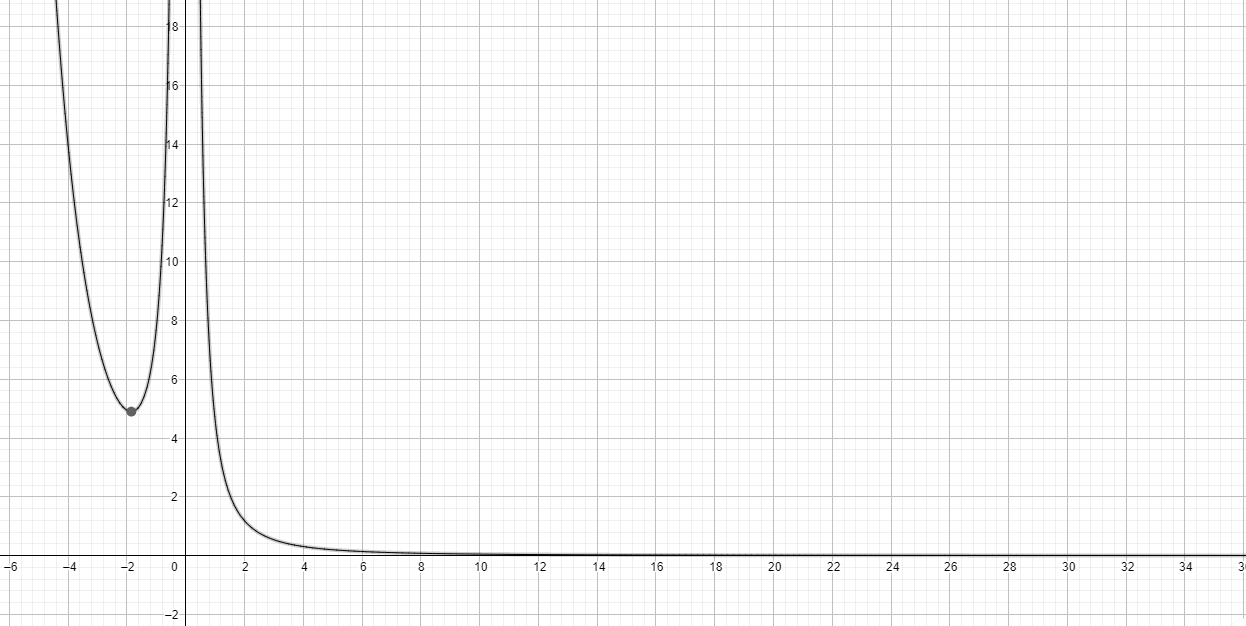
\includegraphics[scale = 0.4]{gra.PNG}
    \end{figure}
    
    entonces para $E > 0$ , no existirá limite superior aunque sí uno inferior para $r$ por lo que se tienen orbitas no acotadas, para $E < 0$ dado que el potencial efectivo es mayor a cero, ese valor es imposible, se podrían tener orbitas cerradas para $r< 0$ pero como eso no es posible pues no hay.
    
    
    
    
    \item ¿Cuando son posibles órbitas circulares? Hallar el periodo de las pequeñas oscilaciones radiales respecto al movimiento circular.
    
    \textbf{Sol:}
    
    El lagrangiano para nuestro potencial es
    
    \begin{equation*}
        L= \frac{1}{2} m (\dot{r}^2 + r^2 \dot{\theta}^2) + \frac{k}{r} e^{-\alpha r}
    \end{equation*}
    
    ahora las ec. de movimiento son
    
    \begin{equation*}
        m r^2 \ddot{\theta} = 0
    \end{equation*}
    
    lo que nos da la conservación del momento angular, y para $r$
    
    \begin{equation*}
        m \ddot{r} - m r \dot{\theta}^2 + k (1 + \alpha r) \frac{e^{-\alpha r}}{r^2} = 0
    \end{equation*}
    
    entonces para tener orbitas circulares se debe tener que $\dot{r}=0$ entonces $\ddot{r} =0$ y así
    
    \begin{equation*}
        r \dot{\theta}^2 = \frac{k}{m} (1 + \alpha r) \frac{e^{-\alpha r}}{r^2}
    \end{equation*}
    
    entonces la velocidad angular necesaria para tener orbitas circulares es:
    
    \begin{equation*}
        \dot{\theta} = \sqrt{\frac{k}{m}(1+\alpha r')} \frac{e^{-\alpha r'/2}}{(r')^{3/2}}
    \end{equation*}
    
    para algún $r'$
    
    y su periodo es
    
    \begin{equation*}
        T = \frac{2\pi}{\dot{\theta}} = \frac{2\pi (r')^{3/2}}{\sqrt{\frac{k}{m}(1 + \alpha r') e^{-\alpha r'}}}
    \end{equation*}
    
\end{enumerate}



%%%3%%%



\item Sea $U(r)$ el potencial arbitrario de un campo de fuerzas centrales.

\begin{enumerate}
    \item Haga la transformación $r=1/u$ y obtenga la ecuación diferencial (de la orbita) para $u(\phi)$.
    
    \textbf{Sol:}
    
    Ya que el momento angular se conserva,podemos escribir
    
    \begin{equation*}
        \dot{\phi} =  \frac{M}{mr^2}
    \end{equation*}
    
    y entonces
    
    \begin{equation*}
    \frac{d}{dt} = \frac{M}{mr^2} \frac{d}{d \phi}
    \end{equation*}
    
    con segunda derivada
    
    \begin{equation*}
        \frac{d^2}{dt^2} = \frac{M^2}{m^2 r^2} \frac{d}{d\phi} \left(\frac{1}{r^2}\frac{d}{d\phi}\right)
    \end{equation*}
    
    y sacando la ec. de movimiento de la lagrangiana del problema anterior
    
    \begin{equation*}
        \frac{d}{dt} \left(m\dot{r}\right)- mr \dot{\phi}^2 + \frac{\partial U}{\partial r} =m\ddot{r}- \frac{M^2}{m r^3} + \frac{\partial U}{\partial r} =0
    \end{equation*}
    
    se tiene que
    
    \begin{equation*}
        m \frac{M^2}{m^2 r^2} \frac{d}{d \phi} \left(-\frac{1}{r^2}\frac{dr}{d \phi}\right) + \frac{M^2}{m r^3} = \frac{\partial U}{\partial r}
    \end{equation*}
    
    ahora sea $u = 1/r$ y $du = - 1/r^2$, entonces
    
    \begin{equation*}
        \frac{M^2 u^2}{m} (\frac{d^2 u}{d \phi^2} + u) = U'
    \end{equation*}
    
    
    
    
    
    \item Obtenga la forma explicita de la ecuación diferencial si $U(r) = -k/r^{\beta}$, donde $k$ y $\beta$ son constantes.
    
    \textbf{Sol:}
    
    Primero derivemos el potencial
    
    \begin{equation*}
        \frac{\partial U}{\partial r} = \frac{k\beta}{r^{\beta + 1}} = k \beta u^{\beta + 1}
    \end{equation*}
    
    entonces por el inciso anterior
    
    \begin{equation*}
    \frac{M^2u^2}{m} \left(\frac{d^2 u}{d \phi} + u\right) = k \beta  u^{\beta + 1}
    \end{equation*}
    
    \begin{equation*}
        \frac{M^2u^2}{m} \left(\frac{d^2 u}{d \phi} + u - \frac{k\beta m u^{\beta -1}}{M^2}\right) = 0
    \end{equation*}
    
    y como $u \neq 0$ $\forall r$,
    
    \begin{equation*}
        \frac{d^2 u}{d \phi} + u - \frac{k\beta m u^{\beta -1}}{M^2} = 0
    \end{equation*}
    
\end{enumerate}



%%%4%%%



\item Una partícula se mueve en dos dimensiones bajo la acción de un campo de fuerzas centrales determinado por el potencial $U(r) = \alpha r^{p} + \beta r^{q}$. Halle las potencias $p$ y $q$ para las cuales es posible una orbita espiral de la forma $r = c \theta^2$, donde c es una constante.

\textbf{Sol:}

Se sabe que

\begin{equation*}
    \theta = \int \frac{M dr}{r^2 \sqrt{2m(E-U(r)) - M^2/r^2}}
\end{equation*}

y para tener la espiral se debe cumplir

\begin{equation*}
    \theta = \sqrt{\frac{r}{c^2}}
\end{equation*}

entonces derivando y sustituyendo el potencial

\begin{equation*}
    \frac{M}{r^2 \sqrt{2m(E - \alpha r^{p} - \beta r^{q} ) - M^2 /r^2}} = \frac{1}{2\sqrt{c^2 r}} 
\end{equation*}

\begin{equation*}
    4 c^2 r^2 + 1 = \frac{2m}{M} (Er^2 - \alpha r^{p +2} - \beta r^{q+2} ) 
\end{equation*}

y así tenemos que

\begin{equation*}
    c = \sqrt{\frac{m E}{2 M}} \hspace{1cm} \frac{2m}{M} (\alpha + \beta) = -1 \hspace{1cm} p = q = -2
\end{equation*}







%%%5%%%



\item \begin{enumerate}
    \item Demuestre que para una partícula de masa $m$ en un campo de fuerzas centrales $V(r) = -k/r$ (problema de Kepler), el vector
    
    \begin{equation*}
        \mathbf{A} = \mathbf{p} \times \mathbf{L} - mk \frac{\mathbf{r}}{r}
    \end{equation*}
    
    conocido como vector de Laplace-Runge-Lenz es una constante de movimiento.
    
    Como el momento angular se conserva
    
    \begin{equation*}
        \frac{d \mathbf{A}}{dt} = \dot{\mathbf{p}} \times \mathbf{L} - mk \frac{\dot{\mathbf{r}}}{r} + mk \frac{\mathbf{r}}{r^2} \dot{r} 
    \end{equation*}
    
    ahora usando que $\dot{p} = - \frac{k}{r^2}\frac{\mathbf{r}}{r}$ y $\mathbf{L} = \mathbf{r} \times m\dot{\mathbf{r}}$
    
    \begin{equation*}
        \frac{d \mathbf{A}}{d t} = - \frac{k}{r^2} \frac{\mathbf{r}}{r} \times (\mathbf{r} \times m \dot{ \mathbf{r}}) - mk \frac{\dot{\mathbf{r}}}{r} + mk \frac{\mathbf{r}}{r^2} \dot{r}
    \end{equation*}
    
    y por la identidad del triple producto cruz
    
    \begin{equation*}
         \frac{d \mathbf{A}}{dt} = -mk  \left(\frac{\mathbf{r}(\mathbf{r} \cdot \dot{\mathbf{r}}) - r^2 \dot{\mathbf{r}}}{r^3} + \frac{\dot{\mathbf{r}}}{r} - \frac{\mathbf{r}}{r^2}\dot{r}\right)
    \end{equation*}
    
    y ya que $\frac{1}{2} \frac{d}{dt} (\mathbf{r} \cdot \mathbf{r}) = \mathbf{r} \cdot \dot{\mathbf{r}} = r \dot{r}$
    
    \begin{equation*}
         \frac{d \mathbf{A}}{dt} = -mk  \left(\frac{\mathbf{r}r\dot{r}-r^2 \dot{\mathbf{r}}}{r^3} + \frac{\dot{\mathbf{r}}}{r} - \frac{\mathbf{r}}{r^2}\dot{r}\right) = 0
    \end{equation*}
    
    por lo tanto $\mathbf{A}$ es una constante de movimiento
    
    \item muestre que este vector pertenece al plano de la orbita.
    
    \textbf{Sol:}
    
    Para demostrar que $\mathbf{A}$ pertenece al plano de la orbita,debemos mostrar que
    
    \begin{equation*}
        \mathbf{A} \cdot \mathbf{L} =0
    \end{equation*} 
    
    entonces
    
    \begin{equation*}
        \mathbf{A} \cdot \mathbf{L} = (\mathbf{p} \times \mathbf{L} - mk \frac{\mathbf{r}}{r}) \cdot L
    \end{equation*}
    
    y como $\mathbf{p} \times \mathbf{L}$ es ortogonal a $\mathbf{L}$ y por definición $\mathbf{r}$ es ortogonal a $L$
    
    
    \begin{equation*}
         \mathbf{A} \cdot \mathbf{L} = \cancel{\mathbf{p} \times \mathbf{L}\cdot L
         }- \cancel{mk \frac{\mathbf{r}}{r} \cdot L} = 0
    \end{equation*}
    
    por lo tanto $\mathbf{A}$ pertenece al plano de la orbita.
    
    
    
    
    
    \item Pruebe que la ecuación de la órbita está dada por
    
    
    \begin{equation*}
        \frac{1}{r} = \frac{mk}{L^2} \left(1 + \frac{A}{mk}\cos{\theta}\right)
    \end{equation*}
    
    \textbf{Sol:}
    
    Sea $\theta$ el angulo entre $\mathbf{r}$ y $\mathbf{A}$, entonces
    
    \begin{equation*}
        \mathbf{A} \cdot \mathbf{r} =\mathbf{p} \times \mathbf{L} \cdot \mathbf{r} - mk \frac{\mathbf{r} \cdot \mathbf{r}}{r} =\mathbf{p} \times \mathbf{L} \cdot \mathbf{r} - mk r=Ar \cos{\theta} 
    \end{equation*}
    
    y por la semiconmutatividad del triple producto escalar
    
    \begin{equation*}
        \mathbf{A} \cdot \mathbf{r} =\mathbf{p} \times \mathbf{r} \cdot \mathbf{L} - mk r=\mathbf{L} \cdot \mathbf{L} - mk r=L^2 - mk r=Ar \cos{\theta} 
    \end{equation*}
    
    por lo tanto despejando
    
    \begin{equation*}
        r (mk + A\cos{\theta}) = L^2 \hspace{1cm} \rightarrow \hspace{1cm} \frac{1}{r} = \frac{mk}{L^2} \left(1 + \frac{A}{mk} \cos{\theta}\right)
    \end{equation*}
    
    \item Determine la relación entre $\mathbf{A}$ y la excentricidad $\epsilon$ de la órbita.
    
    \textbf{Sol:}
    
    La ec. del inciso anterior se puede reescribir de la siguiente forma 
    
    \begin{equation*}
        \frac{\frac{mk}{L^2}}{r} = \left(1 + \frac{A}{mk}\cos{\theta}\right)
    \end{equation*}
    
    la cual es muy parecida a la ec. de la trayectoria para el potencial usado($p/r = 1 +\epsilon \cos{ \theta}$) por lo que podemos decir  que la excentricidad es
    
    \begin{equation*}
        \epsilon = \frac{A}{mk} = \sqrt{1 + \frac{2EL^2}{mk^2}}
    \end{equation*}
    
\end{enumerate}



%%%6%%%



\item Evaluar aproximadamente el cociente entre las masas del Sol y la Tierra, utilizando únicamente las duraciones del año y del mes lunar (27.3 días) y los radios medios de la orbita terrestre ($\num{1.49 e 8}km$) y de la orbita lunar ($\num{3.5e5} km$).

\textbf{Sol:}

Como se vio para el problema de Kepler, el periodo orbital $T$ es
    
    \begin{equation*}
        T= 2\pi a^{3/2} \sqrt{m/ \alpha}
    \end{equation*}
    
    con  $a$ el radio medio de la orbita, $m= \frac{m_i m_j}{m_i + m_j}$ la masa reducida del sistema y $\alpha=G m_i m_j$ 
    
    Supongamos que $m_i >> m_j$, entonces se tiene que
    
    \begin{equation*}
        \left(\frac{T}{2\pi}\right)^{2} = a^3 \frac{\cancel{m_i m_j}}{\cancel{m_i m_j} G (m_i + m_j)} \approx \frac{a^3}{Gm_i}
    \end{equation*}
    
    ahora ya que la masa de la tierra ($m_T$) es mucho mayor a la de la luna ($m_L$) y a su vez la masa del sol ($m_S$) es mucho mayor a la de la tierra, entonces
    
    \begin{equation*}
        \left(\frac{T_{ST}}{2\pi}\right)^{2} = \frac{a_{ST}^{3}}{G m_S}
    \end{equation*}
    
    
    \begin{equation*}
        \left(\frac{T_{TL}}{2\pi}\right)^{2} = \frac{a_{TL}^{3}}{G m_T}
    \end{equation*}
    
    por lo tanto
    
    \begin{equation*}
        \frac{m_T}{m_S} = \left(\frac{T_{ST}}{T_{TL}}\right)^{2} \left(\frac{a_{TL}}{a_{ST}}\right)^{3} =  \left(\frac{365}{27.3}\right)^{2} \left(\frac{\num{3.5e5}}{\num{1.49e8}}\right)^{3} = \num{2.32e-6}
    \end{equation*}
    
    



%%%7%%%



\item Suponga una partícula de masa $m$ que se mueve en el potencial unidimensional $U(x) = A|x|^{n}$, donde A es una constante. Demuestre que el periodo $T$ del movimiento periódico de la partícula depende de su energía E como

\begin{equation*}
    T \propto E^{\frac{1}{n} - \frac{1}{2}}
\end{equation*}


\textbf{Sol:}

Por la conservación de la energía

\begin{equation*}
    E = K + U = \frac{1}{2} m \dot{x}^2 + A |x|^n
\end{equation*}

o bien

\begin{equation*}
    dt = \frac{dx}{\sqrt{\frac{2(E - A|x|^n)}{m}}} \hspace{1cm} \rightarrow \hspace{1cm} t =\frac{m}{2} \int  \frac{dx}{\sqrt{E - A|x|^n}}
\end{equation*}

entonces dada la forma del potencial, el periodo $T$ es

\begin{equation*}
    T (E) = 2 \sqrt{2m}  \int_{-(E/A)^{1/n}}^{(E/A)^{1/n}} \frac{dx}{\sqrt{E - A|x|^n}}
\end{equation*}

ahora sea $|y| = (A/E)^{1/n} |x|$, $dx = (E/A)^{1/n}dy$ y suponiendo que $\int_{-1}^{0} \frac{dy}{\sqrt{1 + y^n}} = 0$

\begin{equation*}
    T = 2\sqrt{2m} (E/A)^{1/n} \int_{-1}^{1} \frac{dy}{\sqrt{E - E|y|^n}} = 2 \sqrt{\frac{2m}{E}} (E/A)^{1/n} \left[ \int_{0}^{1} \frac{dy}{\sqrt{1 - y^n}}  \right]
\end{equation*}

que con el cambio de variable $y^n = u$ se llega a que

\begin{equation*}
    T = \left[2 \sqrt{\frac{2 \pi m}{ A^{1/n}}} \frac{\Gamma (1/n) }{\Gamma(1/2 + 1/n)} \right] E ^{1/n - 1/2} \hspace{1cm} \rightarrow \hspace{1cm} T \propto E^{\frac{1}{n} - \frac{1}{2}}
\end{equation*}





%%%8%%%



\item Una carga puntual $q$ de masa $m$ se mueve (de manera restringida) sobre una circunferencia de radio $R$ en el plano vertical y bajo la acción del campo gravitatorio. Otra carga $q$ está fija en el punto más bajo de la circunferencia. 

\begin{figure}[h!]
    \centering
    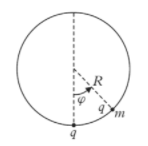
\includegraphics{8.PNG}
\end{figure}

\begin{enumerate}
    \item Encuentre la posición de equilibrio
    
    \textbf{Sol:}
    
    Por ley de cosenos, la distancia entre las 2 cargas está determinada por
    
    \begin{equation*}
        r^2 = R^2 + R^2 - 2R^2 \cos{\phi} 
    \end{equation*}
    
    \begin{equation*}
        = 2R^2 (1 - \cos{\phi}) = 4 R^2 \sin^2{\phi/2}
    \end{equation*}
    
    entonces el potencial del sistema es ($a = kq^2/8mgR^2$)
    
    \begin{equation*}
        U(\phi) = 2mgR \left(\frac{2a}{r} +\sin^2{\phi/2}\right) =2mgR\left( \frac{2a}{\sin{\phi/2}} +\sin^2{\phi/2}\right)
    \end{equation*}
    
    y así (sea $u = \sin{\phi/2}$ )
    
    \begin{equation*}
        \frac{\partial U}{\partial \phi} =2mgR\left(  a \frac{\partial}{\partial \phi}  \frac{1}{\sin{\phi/2}} + \frac{\partial }{\partial \phi} \sin^2{\phi/2}\right)
    \end{equation*}
    
    \begin{equation*}
        = 2mgR \left( a\frac{\partial}{\partial u} \frac{1}{u} \frac{\partial u}{\partial \phi} + \sin{\phi/2} \cos{\phi/2} \right)
    \end{equation*}
    
    \begin{equation*}
        =2mgR \left(\sin{\phi/2} \cos{\phi/2}-a \cos{\phi/2} \csc{\phi/2} \right)
    \end{equation*}
    
    \begin{equation*}
        =2mgR \cot{\phi/2}\left(\sin^2{\phi/2} - a \right)
    \end{equation*}
    
    que tiene como raíces a $\phi = \frac{\pi}{2} (2n+1)$ con $n \in  Z$ y $\phi = 2\sin^{-1}{a}$
    
    \item Encuentre la frecuencia de las oscilaciones pequeñas de la carga móvil
    
    \textbf{Sol:}
    
    recordando que $k = \frac{\partial^2 U}{\partial \phi^2}$, entonces
    
    \begin{equation*}
        k = mR (2\sin^2{\phi/2} + a \csc^2{\phi/2} - 3)
    \end{equation*}
    
    \begin{equation*}
        \omega = \sqrt{\frac{k}{m}} = \sqrt{R(2\sin^2{\phi/2} + a \csc^2{\phi/2} - 3)}
    \end{equation*}
    
    
\end{enumerate}
    
    
    
    
%%%9%%%



\item Halle la frecuencia de las oscilaciones pequeñas del regulador centrífugo. El sistema rota con velocidad angular constante $\Omega$ alrededor del eje vertical, bajo el campo gravitatorio. Considere que 4 varillas articuladas de longitud $a$ son de masa despreciable y que la masa $M$ se desplaza libremente (sin fricción) sobre la varilla vertical.

\begin{figure}[h!]
    \centering
    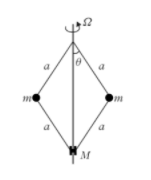
\includegraphics{9.PNG}
\end{figure}

\textbf{Sol:}

Usando coordenadas esfericas

\begin{equation*}
    x  = r \sin{\theta} \cos{\Omega t}
\end{equation*}

\begin{equation*}
    y = r \sin{\theta} \sin{\Omega t}
\end{equation*}

\begin{equation*}
    z = - r \cos{\theta}
\end{equation*}

se puede obtener la lagrangiana

\begin{equation*}
    L = a^2 \dot{\theta}^2 (m+2M\sin^2{\theta}) + ma^2 \Omega^2 \sin^2{\theta} + 2ga (m+M) \cos{\theta}
\end{equation*}

con un potencial $U(\theta) = ma^2 \Omega^2 \sin^2{\theta} + 2ga (m+M) \cos{\theta}$, entonces

\begin{equation*}
    k = \frac{\partial^2 U}{\partial \theta^2} = 2ma^2 \Omega^2 (\cos^2{\theta} - \sin^2{\theta}) - 2ga (m+M)\cos{\theta}
\end{equation*}

por lo tanto

\begin{equation*}
    \omega = \sqrt{\frac{k}{2m+M}} = \sqrt{\frac{2ma^2 \Omega^2 (\cos^2{\theta} - \sin^2{\theta}) - 2ga (m+M)\cos{\theta}}{2m + M}}
\end{equation*}












    
    
    

\end{enumerate}

\end{document}
